\documentclass[14pt]{beamer}
\usetheme{Warsaw}
\usecolortheme{beaver}
\usefonttheme{professionalfonts}

\input{../../preamble}
\usepackage{amscd,amsmath,amssymb,amsthm,graphicx}
\usepackage{paralist}
\usepackage{tabto}
\usepackage[normalem]{ulem}
\usepackage{tikz}
\usepackage{tkz-euclide}
\usetkzobj{all}
\newcommand{\dint}{\displaystyle\int}
\newcommand{\dlim}{\displaystyle\lim}
\newcommand{\dsum}{\displaystyle\sum}

% % % % % % % % % %
\title[Cal I S2015]{MATH 2554 (Calculus I)}
\subtitle{}
\author[Wheeler]{Dr. Ashley K. Wheeler}
\institute{University of Arkansas}
\date{\today}
\logo{}

% % %
\begin{document}
\maketitle

% % %
\begin{frame}
\frametitle{Table of Contents}
\tableofcontents
\end{frame}

% % % % % % % % % % Mon 20 Apr 2015

% % %
\begin{frame}
\section[Week 14]{Week 14: 20-24 April}
\frametitle{Monday 20 April (Week 14)}
\small
\begin{itemize}
\item Computer HW this week: $\oint 5.3-5.4$; next week: $\oint 5.5$
\item Quiz \#14 tomorrow (Tues) in drill -- in class
\item Exam \#4 Friday 24 April covers $\oint 4.6-5.4$ open in class
\item Quiz \#15 next Tues also in class
\item FINAL! Monday 4 May 6-8p OZAR 026
\item dead day review?
\end{itemize}
\end{frame}

% % %
\subsection[$\oint 5.4$ Working with Integrals]{$\oint 5.4$ Working with Integrals}

% % %
\begin{frame}{$\oint 5.4$ Working with Integrals}{Integrating Even and Odd Functions}
\small
Recall the definition of an even function,
\[f(-x)=f(x),\] 
and of an odd function, 
\[f(-x)=-f(x).\]

These properties simplify integrals when the interval in question is centered at the origin.
\end{frame}

% % %
\begin{frame}{\small Integrating Even Functions}
\footnotesize
Even functions are symmetric about the $y$-axis.  So 

\vspace{-0.5pc}
\[\int_{-a}^0 f(x)\ dx = \int_0^a f(x)\ dx\]

\vspace{-0.4pc}
i.e., the area under the curve to the left of the $y$-axis is equal to the area under the curve to the right.

\vspace{-1.1pc}
\begin{center}
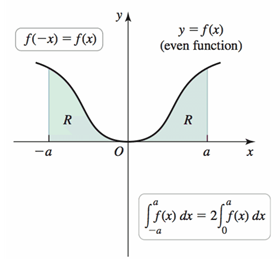
\includegraphics[scale=0.7]{Fig5_50a}
\end{center}

%Hence, $\dint_{-a}^a f(x)\ dx = 2\dint_0^a f(x)\ dx$ for even functions.
\end{frame}

% % %
\begin{frame}{\small Integrating Odd Functions}
\footnotesize
On the other hand, odd functions have $180^{\circ}$ rotation symmetry about the origin.  So

\vspace{-1.25pc}
\[ \int_{-a}^0 f(x)\ dx = -\int_0^a f(x)\ dx\]

\vspace{-0.3pc}
i.e., the area under the curve to the left of the origin is the negative of the area under the curve to the right of the origin.

%Hence, $\dint_{-a}^a f(x)\ dx = 0$ for odd functions.
\vspace{-0.6pc}
\begin{center}
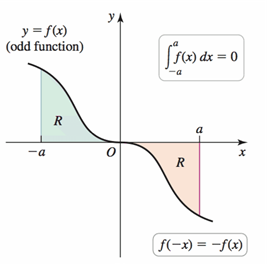
\includegraphics[scale=0.7]{Fig5_50b}
\end{center}
\end{frame}

% % %
\begin{frame}%[t]
\begin{exe}Evaluate the following integrals using the properties of even and odd functions:

\begin{itemize}

\vspace{0.25pc}
\item[1.] $\dint_{-4}^4 (3x^2-x)\ dx$

\vspace{0.5pc}
\item[2.] $\dint_{-1}^1 (1-|x|)\ dx$

\vspace{0.5pc}
\item [3.] $\dint_{-\pi}^{\pi} \sin x \ dx$
\end{itemize}
\end{exe}
\end{frame}

% % %
\begin{frame}{\small Average Value of a Function}
\footnotesize
To find the average of $f(x)$ between points $a$ and $b$, we can estimate by choosing $y$-values $\overline{x}_k$.  If we take $n$ of them, then the average is 
%\[\frac{f(\overline{x}_1) + f(\overline{x}_2) + \dots + f(\overline{x}_n)}{n}\]
%Since $n=\dfrac{b-a}{\Delta x}$, we have
\begin{alignat*}{2}
\frac{f(\overline{x}_1) + f(\overline{x}_2) + \dots + f(\overline{x}_n)}{n} &= 
\frac{f(\overline{x}_1) + f(\overline{x}_2) + \dots + f(\overline{x}_n)}{\left(\dfrac{b-a}{\Delta x}\right)} \\
&= \dfrac{1}{b-a} \left(f(\overline{x}_1) + f(\overline{x}_2) + \dots + f(\overline{x}_n) \right) \Delta x \\
 &= \dfrac{1}{b-a}\sum_{k=1}^nf(\overline{x}_k)\Delta x
\end{alignat*}

The estimate gets more accurate, the more $y$-values we take; as $n \to \infty$, this is \alert{$\dfrac{1}{b-a}\dint_a^b f(x)\ dx$}.
\end{frame}

% % %
\begin{frame}{\small Average Value of a Function}
\small
The average value of an integrable function $f$ on the interval $[a,b]$ is 
\[\overline{f}=\frac{1}{b-a} \dint_a^b f(x)\ dx.\]

\begin{exe} Find the average value of the function $f(x)=x(1-x)$ on the interval $[0,1]$. \end{exe}
\end{frame}

% % %
\begin{frame}{\small Mean Value Theorem for Integrals}
\small
\begin{thm} If $f$ is continuous on $[a,b]$, then there is at least one point $c$ in $[a,b]$ such that 
\[f(c)=\overline{f}=\frac{1}{b-a} \dint_a^b f(x)\ dx.\]
\end{thm}

\bigskip

In other words, the horizontal line $y=\overline{f}=f(c)$ intersects the graph of $f$ for some point $c$ in $[a,b]$. (See Figure 5.54)
\end{frame}

% % %
\begin{frame}%[t]
\small
\begin{exe} Find or approximate the point(s) at which $f(x)=x^2-2x+1$ equals its average value on $[0,2]$. \end{exe}
\end{frame}

% % %
\begin{frame}
\frametitle{HW from Section 5.4}
Do problems 7--27 odd, 31--35 odd (pp.\ 354--355 in textbook)
\end{frame}

% % % % % % % % % % Wed 22 Apr 2015

% % %
\begin{frame}{Wednesday 22 April (Week 14)}
\footnotesize
\begin{itemize}
\item Computer HW this week: $\oint 5.3-5.4$; next week: $\oint 5.5$
\item Exam \#4 Friday 24 April covers $\oint 4.6-5.4$ open in class
	\begin{itemize}
	\footnotesize
	\item open resources but the exam MUST be completed by the end of lecture
	\item The best way to prepare for this exam is to complete the assigned book problems.  Use the same amount of effort and care you used on Exam 3.
	\item CEA: Since the exam is collaborative you have the option to work in class and then finish in my office after.  Please let me know ASAP if this is what you prefer.
	\end{itemize}
\item Quiz \#15 ($\oint 5.5$) next Tues in class
\item FINAL! Monday 4 May 6-8p OZAR 026
\item dead day review details TBA
\end{itemize}
\end{frame}

% % %
\subsection[Exam 4 Review]{Exam 4 Review}

% % %
\begin{frame}
\frametitle{4.6 Mean Value Theorem}
\small
\begin{itemize}
\item Know and be able to state Rolle's Thm and the Mean Value Thm, including knowing the hypotheses and conclusions for both.
\item Be able to apply Rolle's Thm to find a point in a given interval.
\item Be able to apply the MVT to find a point in a given interval.
\item Be able to use the MVT to find equations of secant and tangent lines.
\end{itemize}
\end{frame}

% % %
\begin{frame}
\begin{center}
\Large{You are still responsible for every derivative rule and every derivative formula we have covered this semester.}
\end{center}
\end{frame}

% % %
\begin{frame}
\frametitle{4.7 L'H\^{o}pital's Rule}
\small
\begin{itemize}
\item Know how to use L'H\^{o}pital's Rule, including knowing under what conditions the Rule works.
\item Be able to apply L'H\^{o}pital's Rule to a variety of limits that are in indeterminate forms (e.g., 0/0, $\infty/\infty$, $0 \cdot \infty$, $\infty-\infty$, $1^{\infty}$, $0^0$, $\infty^0$).
\item Be able to use L'H\^{o}pital's Rule to determine the growth rates of two given functions.
\item Be aware of the pitfalls in using L'H\^{o}pital's Rule.
\item \alert{PRACTICE THESE.}  Some of the book problems have non-obvious algebra tricks that simplify an otherwise crazy problem.
\end{itemize}
\end{frame}

% % %
\begin{frame}
\frametitle{4.8 Antiderivatives}
\footnotesize
\begin{itemize}
\item Know the definition of an antiderivative and be able to find one or all antiderivatives of a function.
\item Be able to evaluate indefinite integrals, including using known properties of indefinite integrals (i.e., Power Rule, Constant Multiple Rule, Sum Rule).
\item Know how to find indefinite integrals of the six trig functions, of $e^{ax}$, of $\ln x$, and of the three inverse trig functions listed in the notes.
\item Be able to solve initial value problems to find specific antiderivatives.
\item Be able to use antiderivatives to work with motion problems.
\end{itemize}
\end{frame}

% % %
\begin{frame}
\frametitle{5.1 Approximating Areas under Curves}
\small
\begin{itemize}
\item Be able to use rectangles to approximate area under the curve for a given function.
\item Know how to calculate left Riemann sums, right Riemann sums, and midpoint Riemann sums for a function.
\item Be able to sum a series of numbers written in sigma notation.  You need to know these common sums:  $\dsum_{k=1}^n c = cn$ and $\dsum_{k=1}^n k = \dfrac{n(n+1)}{2}.$
\item Be able to identify whether a given Riemann sum written in sigma notation is a left, right, or midpoint sum.
\end{itemize}
\end{frame}

% % %
\begin{frame}
\frametitle{5.2  Definite Integrals}
\begin{itemize}
\item Be able to compute left, right, or midpoint Riemann sums for curves that have negative components, and understand the concept of net area.
\item Be able to evaluate a definite integral using geometry or a given graph.
\item Know the properties of definite integrals and be able to use them to evaluate a definite integral.
\end{itemize}
\end{frame}

% % %
\begin{frame}
\frametitle{5.3  Fundamental Theorem of Calculus}
\begin{itemize}
\item Understand the concept of an area function, and be able to evaluate an area function as $x$ changes.
\item Know the two parts of the Fundamental Theorem of Calculus and its significance (i.e., the inverse relationship between differentiation and integration).
\item Use the FTC to evaluate definite integrals or simplify given expressions.
\end{itemize}
\end{frame}

% % %
\begin{frame}
\frametitle{5.4  Working with Integrals}
\begin{itemize}
\item Be able to integrate even and odd functions knowing the ``shortcuts'' provided by these functions' characteristics.
\item Be able to find the average value of a function.
\item Know the Mean Value Theorem for Integrals and be able to use it to find points associated with the average value of a function.
\end{itemize}
\end{frame}

% % %
\begin{frame}{Other Remarks on the Exam}
Why you MUST study for this exam, even though it's open:
\begin{itemize}
\item Exam \#3: How many hours did you put into completing it, given all the resources you had?  
\item Exams \#1 and \#2: The notecard alone wasn't enough to help you finish the exam in time.
\end{itemize}
\end{frame}

% % %
\begin{frame}
\footnotesize
Tips for studying efficiently and effectively:
\begin{itemize}
\item Given today's lists of materials you should know for the exam, if you see a topic you don't know then go back to the slides covering that topic first.
\item Review slides for days you missed.
\item Redo the quizzes until you can get a perfect score without looking at the key.
\item Book problems.  Do those problems with the same attention and care you put into Exam \#3.  
\item If you spent 10 hours on Exam \#3 then spend 9 hours studying for Exam \#4, with one hour left for the exam itself.
\end{itemize}	
\end{frame}

\begin{comment}
\end{comment}

\end{document}